\documentclass[12pt,titlepage]{scrreprt}
\usepackage[ngerman]{babel}
\usepackage[utf8]{inputenc}
\usepackage{color}
\usepackage{float}
\usepackage[a4paper,lmargin={2.5cm},rmargin={2.5cm},tmargin={2.5cm},bmargin = {2cm},footskip={1cm}]{geometry}
\usepackage{amssymb}
\usepackage{amsthm}
\usepackage{graphicx}
\usepackage{subfig}
\usepackage{wrapfig}
\usepackage{url}
\usepackage{calc}
\usepackage{overcite} 
\usepackage{amsmath}
\usepackage{amssymb}
\usepackage{tabularx}
\usepackage{siunitx}
\renewcommand\citeform[1]{[#1]}
\usepackage{hyperref}
\hypersetup{
% colorlinks=false,
  pdfborder={0 0 0}
}

% !TEX program = xelatex
\begin{document}
% \include{Title}
\begin{titlepage}

	

\title{Archer-Tracking}
\subtitle{Bewegungstracking für Sportler}
\titlehead{\centering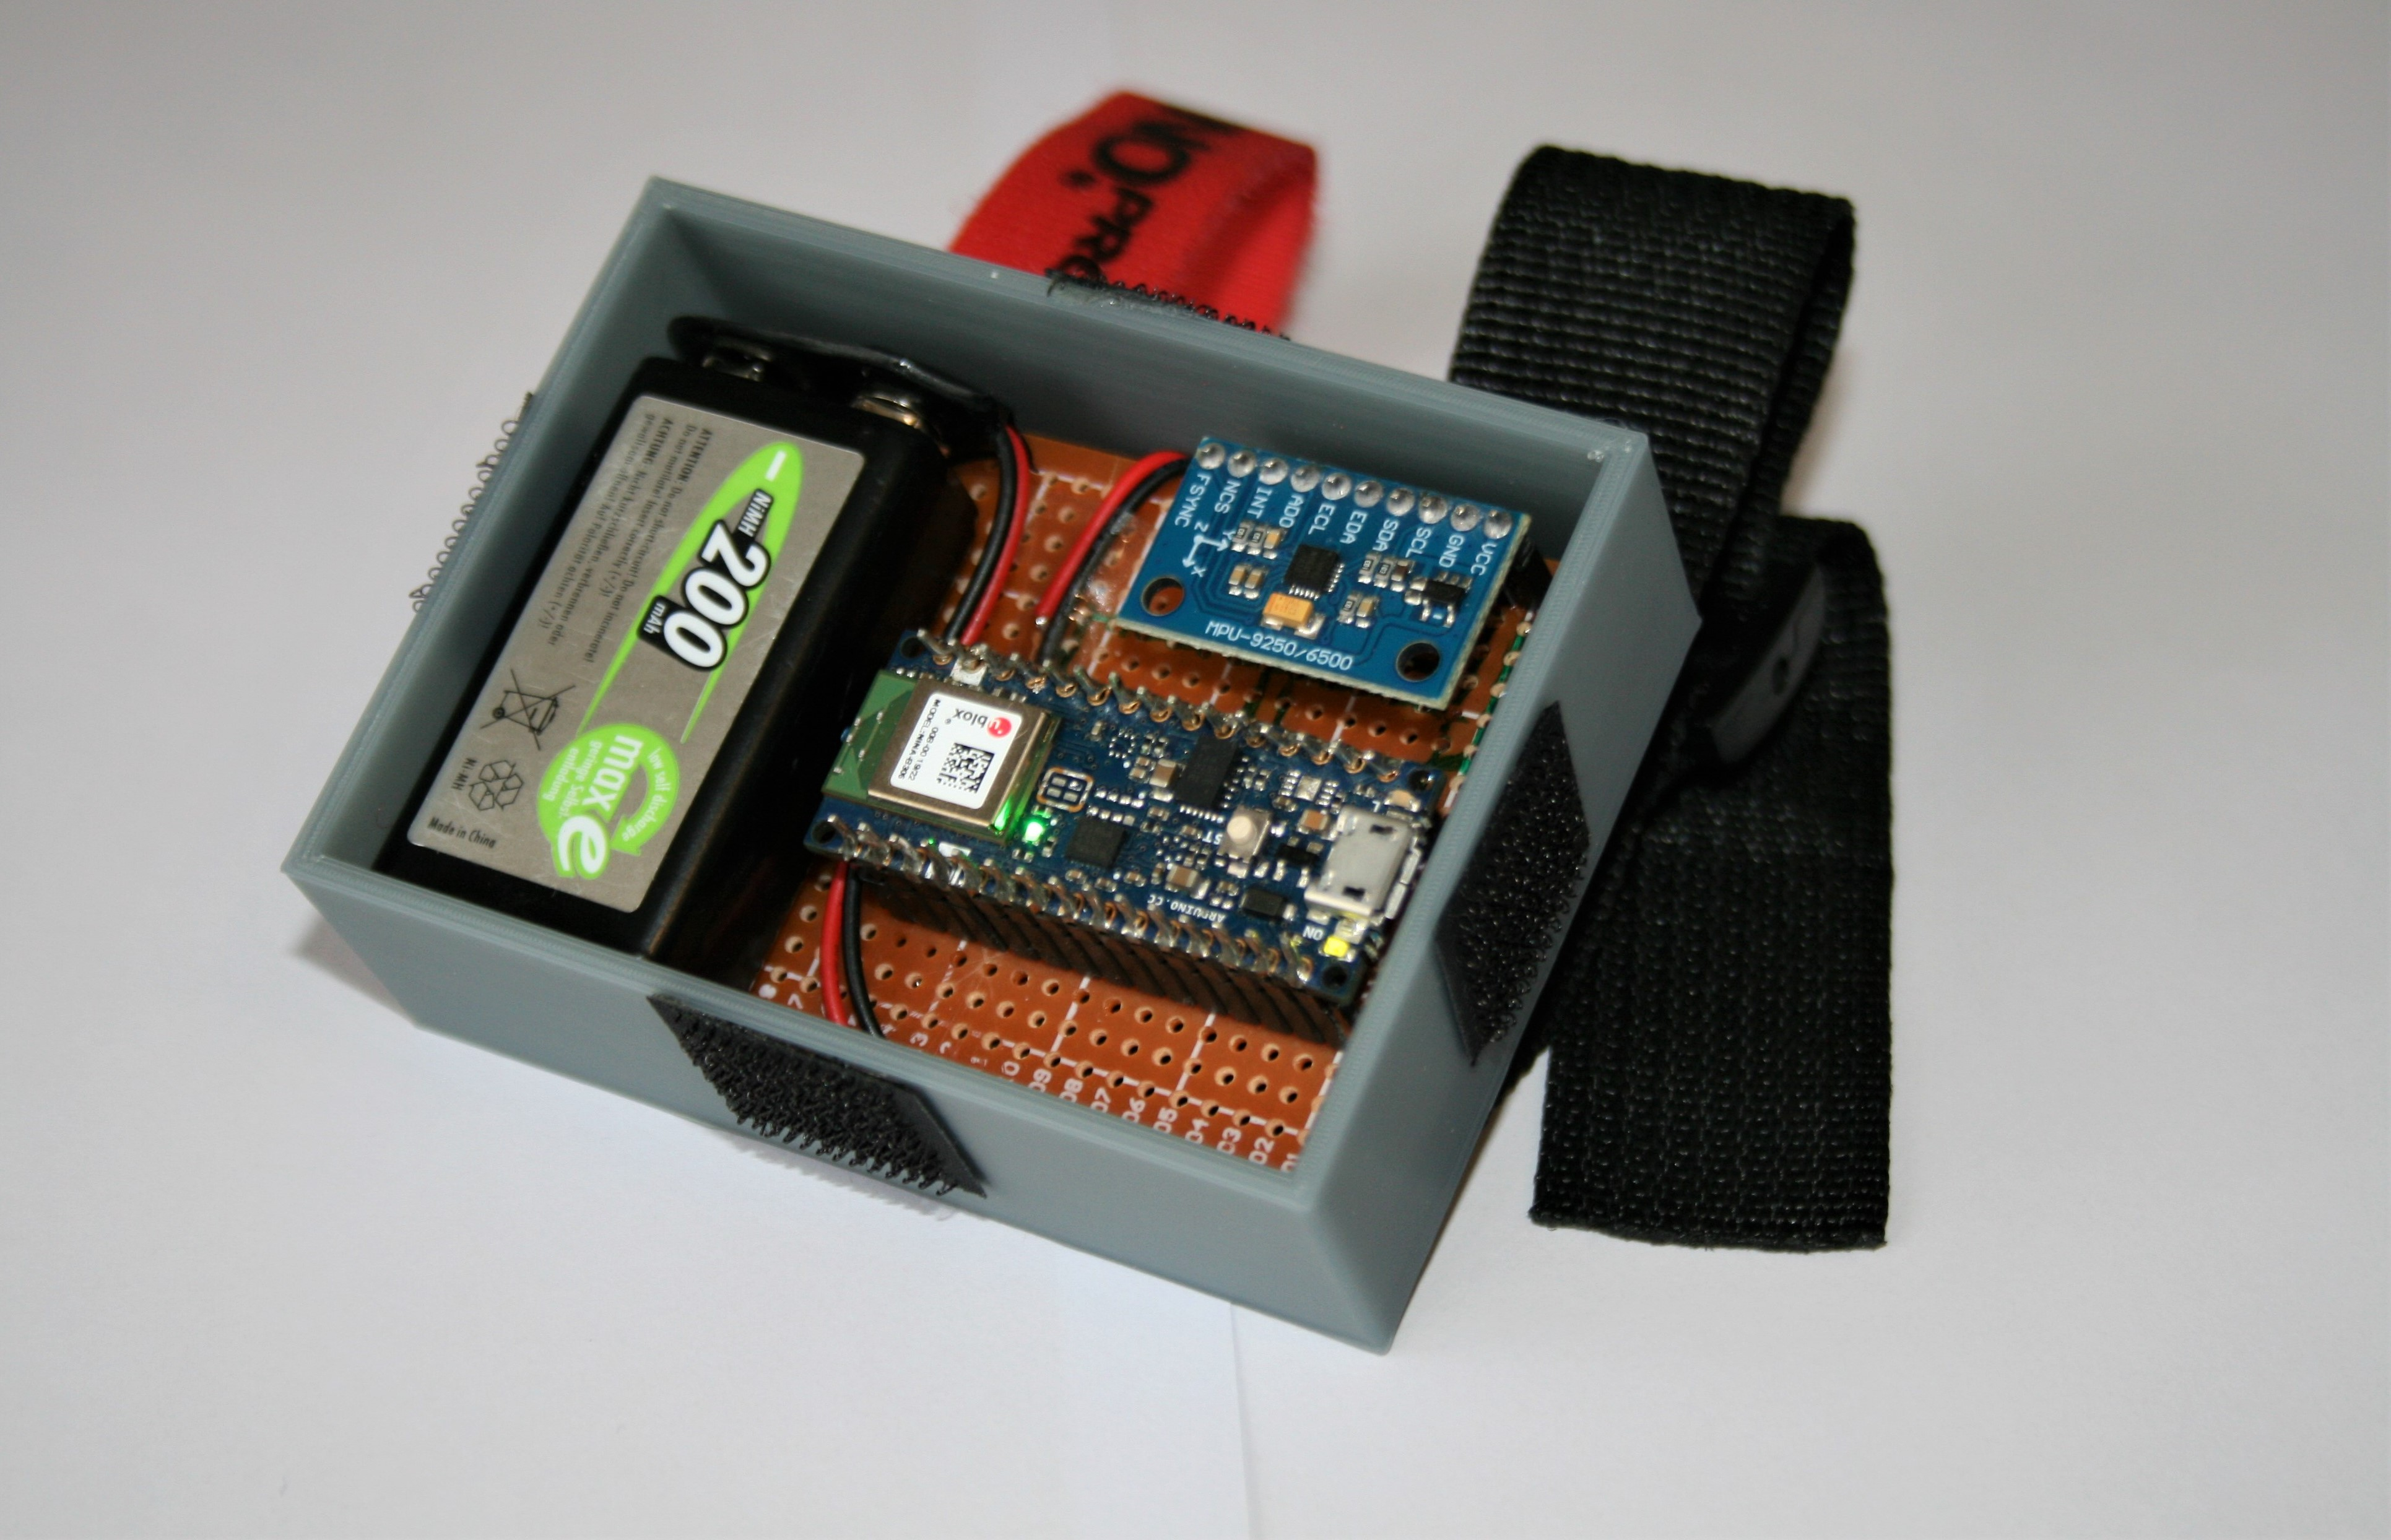
\includegraphics[width=15cm]{Bilder/IMG_9973 (4)}}


\author{Antonio Rehwinkel}

\publishers{Unterstützende Lehrer: Herr Czernohous \\ Herr Dierle \\  \texttt{Emails?} \\
\vspace*{2ex} und Professoren: Hochschule1 \\ Hochschule2\\ \texttt{Emails?}}
%- \\ Schiller-Gymnasium Offenburg}

\maketitle

\end{titlepage}
\tableofcontents
\chapter{Einleitung}
%\subsection{Problemlage}
%Als Bogenschütze bekommt man schnell mit, auf welch hohem Niveau andere Schützen es 
%schaffen, immer wieder dasselbe zu tun. Dies bezieht sich nicht nur auf den allgemeinen 
%Aufbau, bei dem diese Eigenschaft sogar von Nöten ist, sondern auch auf Fehler im Aufbau.\\
%\\
%Da ich selbst schieße und die Möglichkeit hatte in zwei unterschiedlichen Vereinen zu 
%trainieren, ergab sich schnell das Problem, dass meine Schussform drohte schlechter zu 
%werden. Ohne Trainer, der meinen persönlichen Aufbau kannte, konnte ich nicht feststellen, 
%wann ich Fehler wiederholte oder sogar neue einbaute. Eine Lösung musste her, die es mir 
%erlaubte meinen Schussablauf selbst nachzuverfolgen und Unterschiede oder Fehler selbst zu 
%finden.\\
%\\
%Bei Profi-Schützen wird schon seit langem "Ahnliches getan. Mit Hilfe von mindestens zwei 
%Hochgeschwindigkeitskameras und Punkten am Schützen, ist man in der Lage, den 
%Bewegungsablauf eines Schützen zu analysieren und dreidimensional darzustellen.\\
%\\
%Die wohl bekanntesten Aufnahmen werden derzeit vorrangig zum Perfektionieren der 
%mechanischen Ausrüstung und als Lehrmaterial verwendet. Da Profi-Schützen häufig einen 
%nahezu perfekten Aufbau haben, werden die Daten selten zum Korrigieren von Aufbaufehlern 
%eingesetzt.\\
%\\
%Zur Auswertung der Daten ist eine weitere Person von Nöten, die speziell darauf geschult 
%wurde, die erzeugten Daten auszuwerten.\\
%\\
%Die Hochgeschwindigkeitskameras, welche bei den ersten Aufnahmen von Bogenschützen 
%benutzt wurden, sind in der Lage 6000 bis 8000 Fotos in der Sekunde zu schießen. Kameras 
%dieser Qualität kosten selbst heute noch über 100 000 \euro{}.\\
%\\
%Der Raum, den diese Messmethode in Beschlag nimmt, ist ebenfalls nicht zu unterschätzen.
\section{Problemlage}
Bogenschießen, der Sport der perfekten Wiederholung. Je besser ein Schütze seinen Schussablauf wiederholen kann, 
desto einfacher ist es für den Trainer Fehler zu finden und das Visier einzustellen. Sehr gute Trefferbilder sind 
die Folge.\\
Doch was, wenn der Trainer durch Corona-Regelungen oder Solo-Training nicht dabei sein kann? Der Schütze muss sich
selbst kontrollieren, um keine Gewöhnungsfehler einzutrainieren und schlechter zu werden. Ohne Spiegel oder andere 
Hilfsmittel ist dies jedoch kaum möglich. In genau dieser Situation befand ich mich als Schütze im Frühling 2020.\\ 
\\
Bei professionellen Schützen wird der Bewegungsablauf mittels Hochgeschwindigkeitskameras überprüft und selbst kleinste
Fehler werden entdeckt. Dabei liegt der Fokus meistens auf dem Lösvorgang. Dieser ist nur eine kleine Bewegung und 
dauert nur den Bruchteil einer Sekunde.
Benötigt wird dazu jedoch neben Kamera, Licht und Platz häufig auch eine dritte Person, die die
Datenmenge auswerten kann. All dies macht es kleinen Vereinen unmöglich auch nur an ein ähnliches System zu denken.\\
Das Ziel meiner Arbeit ist es, ein System zu entwickeln, das es dem Schützen ermöglicht, seinen eigenen Schussaufbau 
zu sehen und zuverlässig zu bewerten. Damit unterscheidet sich das Ziel meines Systems, ein Full-Body-Tracking, von der
Punktgenauen beobachtung, wie die Kamera es im obigen System beabsichtigt.

\section{Anforderungen}
Der Schütze soll seinen Schussablauf auf Grund der Daten und Visualisierung auswerten und bewerten können.
Da hierbei der gesamte Bewegungsablauf beobachtet wird, benötigt man keine zentrierte, sehr hohe Genauigkeit wie bei der 
Beobachtung des Lösens des Schützen. Somit muss die Genauigkeit der Hochgeschwindigkeitskameras nicht erreicht werden.
\\
Die Anforderungen an mein Projekt sind damit, dass eine kostengünstige Alternative 
geschaffen wird, die wenig Platz benötigt und schnelle Ergebnisse liefert. Dabei müssen diese 
Ergebnisse genau und für jeden verständlich sein.\\
Des Weiteren darf der Schütze auf keinen Fall gestört werden.
Dies wirkte sich bei meiner Idee vor allem auf die Größe, das Gewicht und die 
Datenübertragung aus.\\
\\
Durch Größe und Preis soll es selbst kleinen Vereinen möglich sein, den Bogenschützen zu vermessen und gezielte Hilfe
auch ohne Trainer zu bieten. Auch Privatpersonen könnten sich so ein System sinnvoll zulegen.\\
\\
Entwickelt und gebaut wurde dieses Projekt im Schuljahr 2020/21 von Zuhause aus und wurde 
im Schuljahr 2021/22 weitergeführt.

\chapter{Vorgehensweise}
\section{Möglichkeiten}
Auf meiner Suche hatte ich die Idee, einen Ultraschallsensor am Schützen zu befestigen. Der 
Ultraschallsensor hätte am Boden befestigt werden können, um die Höhe der einzelnen 
Punkte des Schützen zu bestimmen. Ebenfalls wäre eine Kabelführung für schnellere 
Datenübertragung und damit ein günstigerer Preis möglich gewesen. Dieses statische System
hätte allerdings auf einen sich bewegenden Schützen eingestellt werden m"ussen. Ein großer Widerspruch,
lösbar nur durch weitere Technik, die zu kaufen gewesen wäre.
Auch die Verwendung einer günstigeren Kamera wäre möglich gewesen. Dabei vereint man 
allerdings alle Nachteile, die das Kamera-Tracking hat. Man braucht viel Platz und trotz sehr 
günstiger Kameras treibt man die Kosten in die Höhe.
Meine finale Idee war, eine IMU \footnote{Näheres hierzu in \textit{Kapitel 3.2 MPU9250}} und einen 
BLE-Chip\footnote{Näheres hierzu in \textit{Kapitel 4 Bluetooth-Low-Energy}} zu kombinieren. \\
Der IMU sollte mir die Beschleunigsdaten in alle Richtungen liefern, aus dehnen ich die Distanz berechnen wollte.
Als weitere Möglichkeit bot sich an, mittels des IMU die Orientierung des Sensors zu berechnen.


%\subsection{IMU vs Kameratracking}
%Mein Projekt überschneidet sich in seinen Zielen häufig 
mit Tracking das bei VR-Brillen eingesetzt wird. Hier wird
zur Feststellung der Position des Spielers häufig eine 
Kombination aus Kameratracking und Infrarot-LED. \\
Hierbei muss der Spieler die Fernbedienungen festhalten die
die Infrarot-LEDs beinhalten, während die Kameras im Raum 
so verteilt werden müssen das der Spieler immer erkannt wird.\\
Die Neigung des Kopfes und der Hände werden auch hier häufig 
Mithilfe eines IMU bestimmt.\\
\\
Da diese Systeme viel Platz benötigen, viel Geld kosten und 
für die Bildverarbeitung häufig eine große Rechenkraft benötigen
ist dieses System nicht für viele Privatnutzer sinnvoll oder 
bieten einen Bewegungsfreiraum der Sport zu lässt.\\
\\
Die IMU-Sensoren bestehen mindestens aus einem Gyroskop und einem 
Beschleunigungssensor, manche bieten sogar ein Magnetometer an.
Somit sollte es möglich sein, über die
Beschleunigung die Distantz die ein Körper mit diesem Sensor zurück
legt zu messen. Die Neigung und Orientation sind über das Gyroskop 
und Magnetometer sehr genau messbar.\\
\\
Die Vorteile der IMU liegen auf der Hand, sie sind günstig, klein
und leicht. Aus diesen Gründen trägt fast jeder heutzutage 
so einen Sensor bei sich, die meisten Handys haben ihn schon eingebaut.\\
\\
Für mein Projekt benutze ich dennoch einen eigenen IMU, um die
Qualität der Messdaten sicher zu stellen.

\section{Materialsuche}
Es galt nun, zu den genannten Kriterien die passende Hardware zu finden. Um die Bewegungen des 
Schützen nachzuverfolgen, muss ich wissen, wo die einzelnen wichtigen Punkte des Aufbaus 
sind. Dies betrifft beide Arme und die Schultern. Da sich die Arme viel bewegen, schien es mir 
möglich, mithilfe eines günstigen Beschleunigungssensors die Änderungen festzustellen. Bei 
hoher Genauigkeit könnte dieser vielleicht sogar die Bewegungen der Schultern messen.
Um den Schützen nicht zu behindern, ist eine kabellose Verbindung von Vorteil.



%\chapter{IMU vs Kameratracking}
%Mein Projekt überschneidet sich in seinen Zielen häufig 
mit Tracking das bei VR-Brillen eingesetzt wird. Hier wird
zur Feststellung der Position des Spielers häufig eine 
Kombination aus Kameratracking und Infrarot-LED. \\
Hierbei muss der Spieler die Fernbedienungen festhalten die
die Infrarot-LEDs beinhalten, während die Kameras im Raum 
so verteilt werden müssen das der Spieler immer erkannt wird.\\
Die Neigung des Kopfes und der Hände werden auch hier häufig 
Mithilfe eines IMU bestimmt.\\
\\
Da diese Systeme viel Platz benötigen, viel Geld kosten und 
für die Bildverarbeitung häufig eine große Rechenkraft benötigen
ist dieses System nicht für viele Privatnutzer sinnvoll oder 
bieten einen Bewegungsfreiraum der Sport zu lässt.\\
\\
Die IMU-Sensoren bestehen mindestens aus einem Gyroskop und einem 
Beschleunigungssensor, manche bieten sogar ein Magnetometer an.
Somit sollte es möglich sein, über die
Beschleunigung die Distantz die ein Körper mit diesem Sensor zurück
legt zu messen. Die Neigung und Orientation sind über das Gyroskop 
und Magnetometer sehr genau messbar.\\
\\
Die Vorteile der IMU liegen auf der Hand, sie sind günstig, klein
und leicht. Aus diesen Gründen trägt fast jeder heutzutage 
so einen Sensor bei sich, die meisten Handys haben ihn schon eingebaut.\\
\\
Für mein Projekt benutze ich dennoch einen eigenen IMU, um die
Qualität der Messdaten sicher zu stellen.
\chapter{Hardware}
\section{Arduino Nano 33 BLE}
Der Arduino Nano 33 BLE ist wie der Name schon sagt ein Prozessor aus dem Hause Arduino
der Nano Reihe. Was diesen von der normalen Nano-Reihe unterscheidet ist der BLE-Chip
NINA-b3(nRF52840) auf seinem Rücken. Dieser Chip ermöglicht es dem Arduino über 
Bluetooth 5.0, auch genannt Bluetooth-Low-Energy, mit allen anderen Bluetooth-Geräten ab 
der Bluetooth Version 4.0 kabellos zu kommunizieren.\\
\\
\begin{tabularx}{0.8\textwidth}{l|X}
Eigenschaft & Daten \\
\hline
Memory & 1MB Flash | 256 KB SRAM \\ 

Interfaces & $I^2C$, SPI, \dots \\

Volt & Input: 4,5 - 21 V | Output: 3,3 V\\
\end{tabularx}
\\
\\
Der Arduino ist aufgrund seines BLE-Chips, der I²C-Verbindungsmöglichekit und der 
Output-Volt Zahl von 3,3 Volt der richtige Prozessor für dieses Projekt. Auch die 
kleinen Maße und das geringe Gewicht spielen ihm nur Pluspunkte ein.
\section{MPU9250}
Für eine genaue Datenlage sorgt in meinem Projekt der Multi-Chip MPU9250. Dieser ist mit 
einem 3-Achsen Beschleunigungssensor, einem 3-Achsen Gyroskop Sensor und einem 3-Achsen 
Magnetometer ausgerüstet. Damit bietet er neun Freihtsgrade (9 Degrees of Freedom) und gehört zu der Gruppe der 
Inertialen Messeinheiten\footnote{IMU bzw. Inertial Measurement Unit}.
Alle Sensoren erhielzen eine Kalibrierung innerhalb der 
Firma und können einen Selbsttest bei Benutzung vollziehen. Der Sensor benötigt nur 2,4 bis 3,6 Volt während 
des Betriebs. In der Tabelle sind die Datenpins und die Genauigkeit der Sensoren notiert.\\
\\
\begin{tabularx}{0.8\textwidth}{l|X|XX}
Sensoren & Datenübertragung & Empfindlichkeit                                     \\
\hline
Gyroskop & 3 * 16bit ADCs & $\pm250°/\sec$, $\pm500\sec$, $\pm1000°/\sec$, $\pm2000°/\sec$\\ 
\hline
Beschleunigungssensor & 3 * 16bit ADCs & $\pm2g$, $\pm4g$, $\pm8g$, $\pm16g$\\
\hline
Magnetometer & 3 * 16bit ADCs & full-scale range of $\pm$\SI{4800}{\milli\tesla\meter}T \\
\hline
Übertragung & $I^2C$, SPI, \dots & \\
\end{tabularx}
\\
\\
Die Daten werden über den I²C-Bus vom Arduino abgefragt. Die Abtastrate beträgt hierbei 
mögliche 400kHz. Dabei werden alle Sensoren abgefragt und die Daten versendet.
Durch die geringe Größe des Chips (150mm*250mm), dem geringem Energieverbrauch (3,5mA wenn 
alle Sensoren ausgelesen werden), der hohen Genauigkeit und der Geschwindigkeit der 
Datenübertragung ist dieser Sensor perfekt für dieses Projekt. Der verbaute
DMP (Digital Motion Processor) wird ebenfalls verwendet und filtert die Daten mit einem
Low-Pass-Filter.


\section{Stromverbrauch}
Der Stromverbrauch wurde mit einem Multimeter am Batterieanschluss in
verschiedenen Modi gemessen. Die Ergebnisse stehen in der Tabelle:\\
%Tabelle: Werte: 
%200mA Auslösung:

%BLE aus: 5
%BLE an: 10.2
%BLE Verbunden: 13
%MPU9250 an: 5
%Bereich: 200 | Auflösung : 0,1 uA | +-1% des Messwerts +- 2 Ziffern
%Quelle:https://github.com/Escape9002/ArcherTracking/issues/5

Der Stromverbrauch lässt so berechnen und erleichter die Korrekte Batterie-Wahl.
\\
Die Verwendeten Formeln: 
\begin{equation}
    $$
    P = U / I
    Ah / V = Wh
    Wh / W = t --> (U*I*t) / U*I = t
    $$
\end{equation}
So verbraucht der Arduino:
\begin{equation}
    $$
    0,005 A * 7,4 V = 0,037 W
    $$
\end{equation}
\\
Die Verschiedenen Batterien-Typen stehen in der folgenden Tabelle:\\
\begin{tabularx}{0.8\textwidth}{l|X|X|X|XX}
    Typ & Laufzeit(in Stunden) & Gewicht & Cut-Off-Spannung & Differenz\\
    \hline
    9V & 40 & 0,05Kg &7.2V & $9-7.2 = 2,8$\\
    \hline
    CR2025 & 12 & 0,0025Kg & 2V & $3-2 = 1$\\
    \hline
    2 * CR2025 & 48,6 & 0,005Kg & 2V & $6-2 = 4$\\
\end{tabularx}
%Tabelle
%9V : 40h, 0,05 KG, CutoffVol: 7.2V (9-7.2 = 2,8)
% CR2025 : 12h , 0,0025 Kg, CutoffVolt: 2V (3-2 = 1)
% CR2025 * 2 = 48,6 h, 0,005 Kg, CutoffVolt: 2V (6-2 = 4)
\\
Um eine Stromversorgung des Arduinos sicher zu stellen benötigt man 2 Knopfzellen
des Typs CR2025.Dennoch hat die Knopfzelle CR2025 nicht nur eine bessere 
Laufzeit sondern ebenfalls weniger Gewicht, weniger Platz und eine bessere 
Differenz zwischen Cut-Off-Spannung zu angenotener Spannung.
\\
Gegen das umrüsten auf die Knopfbatterie spricht einzig der Umweltschutz. 
Denn im Gegensatz zu 9-Volt-Batterien gibt es keine Akkus für Knopfzellen.

\chapter{Bluetooth-Low-Energy}
Mit Bluetooth 5.0 wurde eine neue übertragunsweise zu 
Bluetooth hinzugefügt. Diese nennt sich Bluetooth-Low-Energy und zeichnet
sich durch einen geringen Stromverbrauch und dennoch einem höherem 
Datendurchsatz aus. \\
\\
Bluetooth sendet Daten in Paketen. Hierbei ist bei Bluetooth-Low-Energy
(zukünftig BLE) der Sender als Server ausgewiesen und der Empfänger als Client.\\
\\
Die Server bieten ``Services'' an die mit ``Characteristics'' befüllt sind.
So bietet mein Arduino den Service ``MPU9250'' an mit dem Characteristis ``Accl'', ``Gyro''
und ``Mag''.\\
Der Nachteil dieser Verteilung der einzelnen Daten besteht hierbei in der Zeit die für die
Abfrage gebraucht wird. Jede Characteristic muss einzeln abgefragt werden, hierbei kann ein
Großteil des Datensatzes des MPU9250 verloren gehen.\\
\\
Laut Dokumentation beträgt der Maximale Datensatz von BLE 244 Bytes pro Paket bei 
aktiviertem DLE. Diese Funktion ließ ich ausgeschaltet, wodurch ich Maximal
27 Bytes pro Paket versenden kann. Dieses Problem erklärt ebenfalls weshalb die Sensor-Daten
auf verschiedene Characteristics aufgeteilt werden. Alle Daten passen nicht in ein einzelnes
zu versendendes Paket. \\
\\

\section{Datengröse}
Die Daten werden als String versendet, diese werden von Arduino mit einer
Null Terminiert. \\
\\
Die Größer der Sensordaten beträgt:\\
\textit{Vorkommastellen (3) + Komma (1) + Dezimalstellen (2) + Terminierung (1) = 7 Char}\\
\\
1 Char entspricht 1 Byte, somit gilt:\\
\textit{
9 Sensoren * 7 Byte = 63 Byte \\
63 Byte / 27 Byte = 2,3 Datenpakete pro alle Sensoren
}\\
\\
Somit brauche ich für das Senden aller Sensoren mindestens 3 Characteristics.


\section{Datendurchsatz per BLE}
%Quelle:
%https://www.novelbits.io/bluetooth-5-speed-maximum-throughput/
%--------------------------------------------------------------

Das Sendeprotokoll von Bluetooth schreibt vor, das ein Datenpaket von
leeren Datenpaketen eingepackt wird, ebenso ist eine kurze Wartezeit vorgeschrieben. 
Diese beträgt 150 Mikrosekunden und wird abgekürt mit IFS.
Der Arduino Nano unterstützt 2Mbps bei der BLE-Übertragung, dies ist also die Datenrate.\\
\\
Somit beträgt die optimale Sendezeit pro Datenpaket:\\
\textit{Zeit = Sendedauer[Leer] + IFS + Sendedauer[Voll] + IFS\\
Sendedauer[Leer] = Leerespacket / Datarate}\\
\\
Für mich heißt das:\\
\textit{Leerespacket = 2 + 4 + 2 + 3 = 11 Bytes * 8 = 88 bit}\\
\\
und die Sendezeit für das leere Paket beträgt damit:\\
\textit{Sendedauer[Leer] = 88 bit / 2Mpbs = 44 Mikro-Sekunden}\\
\\
Für ein volles Datenpaket brauche ich:\\
\textit{2+4+2+4+27+3 = 42 Byte * 8 = 336 bit\\
Sendedauer[Voll] = 336 bit / 2Mbps = 168 Mikro-Sekunden}\\
\\
Für ein gesamtes Datenpaket brauche ich somit mindestens:\\
\textit{Zeit = 44 + 150 + 168 + 150 = 512 Mikro-Sekunden}\\
\\
beziehungsweise 0,512 Millisekunden. Die maximal erreichbare Datenübetragungs-Frequenz
liegt bei 512Hz.

%-----------------------------------------------------------------

\section{Tatsächliche Übetragunsgeschwindigkeit}
Die ausgerechnete Datenrate kann in der Praxis kaum erreicht werden, weshalb ein Test zur 
tats"achlichen Datenrate Pflicht ist. Gemessen wurde 


\section{Analyse}
Da der Schussablauf eines Bogenschützen viele Stationen mit verschiedenen Bewegungen 
beinhaltet, fällt es häufig sogar den Trainern schwer, zwischen einem technisch guten
oder schlechten Schuss zu unterscheiden.\\ 
Somit galt es einen Punkt zu finden, bei dem Fehler auffällig sind, so dass ich die Daten auch in 
der Praxis nachvollziehen kann.\\
\\
Eine interessante Bewegung stellt vor allem der Zugarm des 
Schützen dar. Der Auszug verläuft nahezu linear, der häufigere Fehler 
an dieser Stelle versteckt sich in der Höhe des Zugarms. 
Um diese zu messen, muss man die Erdanziehungskraft der Z-Achse herausrechnen.\\
Möglich ist ebenso, die Neigung des Armes über die Euler-Winkel zu berechnen. Sollte 
der Arm zu hoch sein, wird sich die Ausrichtung des Sensors stark verändern, so wie 
die zurückgelegte Distanz in Z-Richtung.\\
\\
Um den vollen Bewegungsablauf eines Schützen zu tracken, wird an jedem Körperteil ein Sensor
benötigt. Dies ermöglicht nicht nur das gegenseitige Überprüfen auf Sinnhaftigkeit der Orientation
(menschliches Skelett hat beschränkte Bewegungsfreiräume), sondern auch die Klassifizierung der 
einzelen Schuss-Abläufe könnte, auf Grund von mehr Daten, genauer Ablaufen.\\ 
\\
Der MPU9250 bietet 9 Freiheitsgrade (Degrees Of Freedom - DOF). Aus welchen diese bestehen, wird
im Kapitel zum MPU9250 erläutert. Diese Freiheitsgrade lassen es zu, die Distanz 
die der Sensor sich bewegt, zumindest in der Theorie, zu berechnen. Die Orientierung des Sensors 
und damit die Orientierung des Körpers an der er befestigt ist, kann man genau messen und berechnen. \\
\\
So ist eine Darstellung als 3D-Modell möglich, an der der Schütze seine Fehler sieht und Unterschiede
zu vorangegangen Schüssen hervorgehoben werden. \\
Denkbar wäre eine Klassifizierung der einzelnen Schüsse, um, wie in einem Videospiel, die Genauigkeit
der Wiederholung in Prozent anzugeben. Interessant wird es, sobald mehrere Schützen Datensätze
ihrer Schüsse vergleichen. Unterschiede werden ersichtlich, genau wie Gemeinsamkeiten. \\
\\

Dieses Kapitel beschäftigt sich folgenden mit der dreidimensionalen Visualisierung.

\section{Integrale}
Die Distanz, berechenbar aus den Werten des Beschleunigungssensors, kann uns die Differenz zwischen einem Startpunkt
und dem jetzigen Punkt des Sensors berechnen. Durch die drei Achsen meines Beschleunigungssensors ginge dies sogar in alle Richtungen. Damit 
könnte man ein Modell erzeugen, das den betreffenden Punkt in die einzelnen Richtungen verschiebt, bis der finale
neue Standort des Sensors erreicht wird. \\ 
\\ 
Um die Distanz aus der gemessenen Beschleunigung zu berechnen,
fand ich zwei verschiedene Formeln. Die wohl bekannteste Umrechnung 
benutzt Integrale, die zweite Formel ist die der gleichm"aßigen 
Beschleunigung.\\
\\
Die Integration wird von allen mir bekannten Forschungen verwendet. 
Man muss eine Doppelintegration
ausführen um von Beschleunigung auf Distanz zu kommen, hierbei verwandelt 
sich das Rauschen des Sensors in Drift und so einen exponentiell steigenden
Fehler. \\ 
Die gleichmäßige Formel kann im Gegensatz zum Integral, nur positive 
Beschleunigungen verwerten, hat in den Tests allerdings 
deutlich genauere Werte und einen geringeren Fehler bei Stillstand 
aufgezeigt. \\
\\
Als Zeit wird die Frequenz, mit der der Sensor Daten misst, 
genommen. Hierfür wird die Frequenz in Zeitabschnitte umgerechnet, mit 
der die Formeln letzendlich arbeiten. Den Testaufbau und Durchführung 
sehe sie im Kapitel \textit{ 7.1 Distanz-Testaufbau}.
\subsection{Gleichmäßige Formel}
Die angepasste Formel f"ur gleichm"aßige Beschleunigung berechnete
die Distanz in meinen Versuchen mit einer Genauigkeit von
$\pm8$ cm auf 30cm Teststrecke.\\
Die physikalische Formel für Bewegungen mit einer Anfangsgeschwindigkeit lautet 
$s + v * t  + a * t^2 * 0.5$,
allerdings wurden mit dem leicht verändertem Weg-Zeit-Gesetz $s + a * t^2 * 0.5$ 
bessere Testergebnisse erzielt.\\
Da die negative Beschleunigung den Wert der Distanz wieder nullierte,
wurden zu dieser Formel nur positive Distanzmessungen zugelassen.\\
Hier der Code-Ausschnitt:
\begin{verbatim}
    if (acc > 0) {
    t = (freq / 1000); //hz is not time but frequenzy

    distance = (distance) + (acc * (t * t) * 0.5);
    velocity = acc * t;
    }
\end{verbatim}
F"ur die Tests wurde dieser Code statt der BLE-"Ubetragung auf dem Arduino ausgef"uhrt. 

\subsection{Integral}
Die Berechnung der Distanz über Integrale ist der Standard 
in der Wissenschaft. Beim integrieren meiner Sensordaten ist zu beachten, 
das beim mathematischen Integrieren die zu berechnenden Werte gegen den Limes 
laufen können. Da ich nur begrenzete Datenmengen zur Verfügung habe, ist dies 
nicht möglich, wodurch allein das Integrieren Fehler erzeugt. Ebenfalls wird das 
Rauschen meines Sensors nicht beachtet und aufaddiert. Da ich zwei mal integrieren 
muss, ist dieser Fehler in der Distanz exponentiell.\\
\\
Die Testergebnisse ergaben einen Fehler von $\pm15$cm auf einer Strecke
von 30cm. Ebenso war das Ergebnis sofort in Zentimetern, statt wie erwartet in Metern. 
Wurde der Sensor zurückbewegt an seinen Startpunkt, sank
der Wert jedoch wieder auf Null ab. Somit kann man schließen,
dass das Ergebniss nur falsch skaliert ist.\\
Dieser Fehler wurde noch nicht behoben. \\
Ein klarer Vorteil dieser Rechnung zeigt sich schon beim Test,
die Formel funktioniert auch für negative Beschleunigungen.
Der Wert sinkt am Ende der Teststrecke nicht ab, sondern bleibt
auf seinem hohen Wert.\\
Folgend der Code-Ausschnitt der Integral-Rechnung:
\begin{verbatim}
    t = (freq / 1000); // hz to time

    velocity = t * ((acc + accOld) / 2) + velocity;
    accOld = acc;
    distance = t * ((velocity + velocityOld) / 2) + distance;
    velocityOld = velocity;  
\end{verbatim}

\section{Orientierungen}
Um die Orientierung des Sensors zu berechnen geht man auf die Grundaussagen der Sensoren zurück. Der 
Beschleunigungssensor gibt die G-Kräfte an, daraus lassen sich Rückschlüsse über die Orientierung 
der Pitch- und Roll-Achse ziehen. Das Gyroskop gibt Drehmoment-Werte zurück, worüber sich der Beschleunigungssensor
überprüfen lässt und eine Drehung um die Yaw-Achse messbar macht. Das Magnetomenter setzt schließlich alle Werte in
Relation zum Erdmagnetfeld und kann sowohl das Gyroskop als auch den Beschleunigungssensor überprüfen. Diese Überprüfung
findet über Filter statt, in meinem Projekt verwende ich hierfür den AHRS-Filter\footnote{Der AHRS-Filter 
ist ein erweiterter Kalman-Filter. Er passt seine Fehlerwerte über Zeit dem Drift der Sensorik an und bietet so auch 
auf lange Zeit gute Ergebnisse.}. Der AHRS-Filter fusioniert die Daten in eine verwendbar Orientierung.\\
Für die Darstellung der Orientierung im Dreidimensionalen Raum gibt es mehrere Ansätze, die zwei bekanntesten 
sind wohl die Euler-Winkel und die Quaternionen. Die Vor- und Nachteile werden im folgenden erläutert.
\subsection{Euler-Winkel}
Bei Euler-Winkeln wird das Objekt um die einzelnen Achsen in einer festeglegten Reihenfolge gedreht. Sollten hierbei 
nach einer Drehung zwei Achsen aufeinander liegen, entseht der sogenannte \textit{Gimbal-Lock} und die Darstellung
der Bewegung findet fehlerhaft statt. Für reele Systeme wie Gimbal an einer Drohne ist dieser Fehler vernachlässigbar,
da er nur selten vorkommt und die Euler-Winkel den tatsächlich benötigten Drehwinkeln der Motoren entsprechen.
Da ich jedoch keine Motoren ansteuern muss, steht vor allem der Fehler im Mittelpunkt und ist der Grund, das ich nicht
die Euler-Winkel verwende.  

\subsection{Quaternionen}
Um die Position eines Körpers im dreidimensionalen Raum darzustellen reichen drei Koordinaten, 
die Möglichkeit der Orientierung verlangt jedoch nach einer vierten Koordinate und damit vier Dimensionen. 
Die Quaternionen stellen diese vierte Koordinate dar. Quaternionen finden damit im vierdimensionalen Raum statt
und sind damit für wenige Menschen vollständig nachvollziehbar. Ein Überprüfen der Rohdaten fällt hiermit für mich aus.
Allerdings schaffen es die Quaternionen durch diese weitere Dimension jegliche Orientierung im Raum darzustellen ohne
etwas ähnliches wie einen \textit{Gimbal-Lock} zu erzeugen. Die Vollständige Erklärung der Quaternionen sprengt momentan
leider meinen Wissenstand. Die einfache Eingabe meiner Daten in fast alle läufige 3D-Visualisierungsprogramme und 
der fehlende \textit{Gimbal-Lock} sind der Grund für mich, zukünftig die Quaternionen zu verwenden.

\chapter{Software}
Die Anzeige für Daten erfolgt am Handy, hier habe ich genug Rechenpower
nicht nur Nachkommastellen genau zu berechnen, sondern kann ebenfalls 
visuelle Darstellungen anzeigen. Die Daten werden hierfür über das bereits
erklärte BLE an das Handy gesendet.
\section{Datenübertragung}
\input{Datenübertragung}
\section{Android-App}
Zur Erstellung der Android-App wurde AppInventor(\url{https://appinventor.mit.edu/}) und 
die BLE-Extension verwendet.\\
Geschrieben wurde das Programm von mir. Ideen und Anregungen wurden in verschiedensten 
Foren gefunden. \\
\\
Beim Start der App wird man aufgefordert Bluetooth und GPS anzuschalten, das GPS
ist nach Android-Richtlinien zu aktivieren. Danach kann man nach verschiedenen
Geräten scannen und sich mit diesen zu verbinden. Erfolgt die Verbindung mit einem
falschen Gerät schließt sich die App. Nach der Verbindung wird sofort die Übertragung 
gestartet.\\
Das empfangene Datenpaket muss vor der Verarbeitung in die einzelnen Daten
aufgespalten und von String zu Float-Werten, besser Double-Werten gepaarst werden.
Diese werden in ein Array gespeichert welches später
die einzelnen aktuellen Werte ausgeben kann.\\
\\
Es gibt insgesamt 3 Möglichkeiten die Daten anzeigen zu lassen.

\subsection{Rohdaten}
Die gelesenen Daten werden direkt im Textformat auf dem Bildschirm ausgegeben.
Der Zeitunterschied zwischen Datenpaketen wird in Millisekunden auf dem Bildschirm
angezeigt.
Es ist möglich die Daten gleichzeitig aufzuzeichnen.

\subsection{Graph}
   \begin{minipage}{0.5\textwidth}
        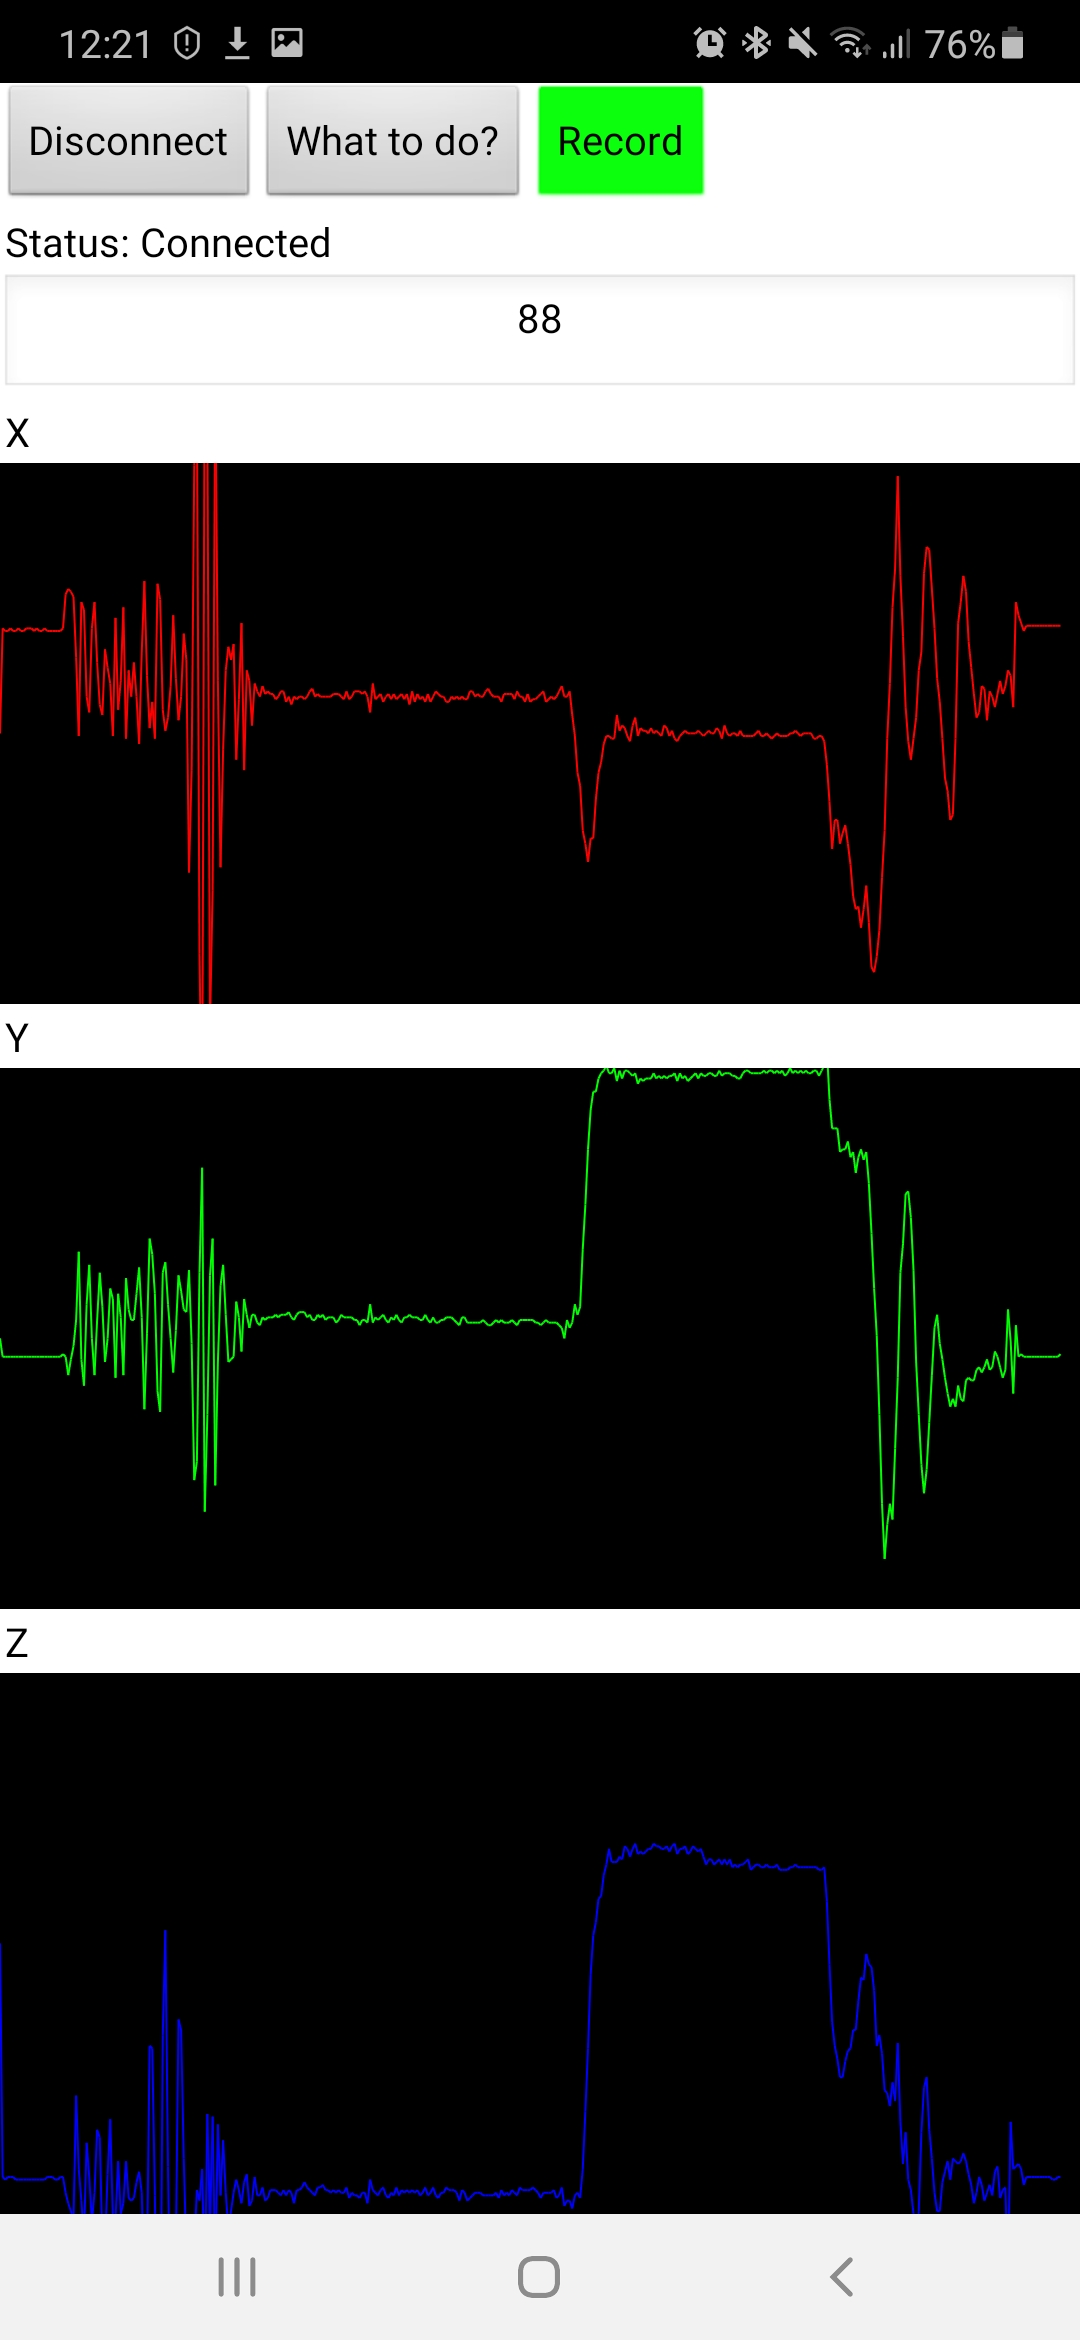
\includegraphics[height=10cm]{Bilder/Graph.jpg}
    \end{minipage}
    \hfill
    \begin{minipage}{0.5\textwidth}
        Die Beschleunigungs-Daten werden in einem Graph dargestellt, hierzu werden sie zuerst in ein
        Array geschrieben. Aus diesem Array erzeugt das Programm in einem vorgegebene Bereich
        die Datenpunkte, die aufgrund ihrer Masse wie ein Liniendiagramm aussehen.\\
        Neue Daten werden rechts geschrieben, während die alten Daten nach Links aus dem
        Bildschirm verschwinden.\\
        Der Zeitunterschied zwischen Datenpaketen wird in Millisekunden auf dem Bildschirm
        angezeigt.
        Es ist möglich die Daten gleichzeitig aufzuzeichnen.\\
    \end{minipage}
\\

\subsection{Animation}
Hier wird die Distanz aus den Beschleunigungsdaten berechnet und mithilfe eines Punktes
visualisiert. Benutzt werden hierfür die X- und Y-Achse. 
Die Rechnung ist in Kapitel `` 5.4.1 Gleichmäßige Formel'' beschrieben.

\subsection{Aufgezeichnete Daten}
    \begin{minipage}{0.5\textwidth}
        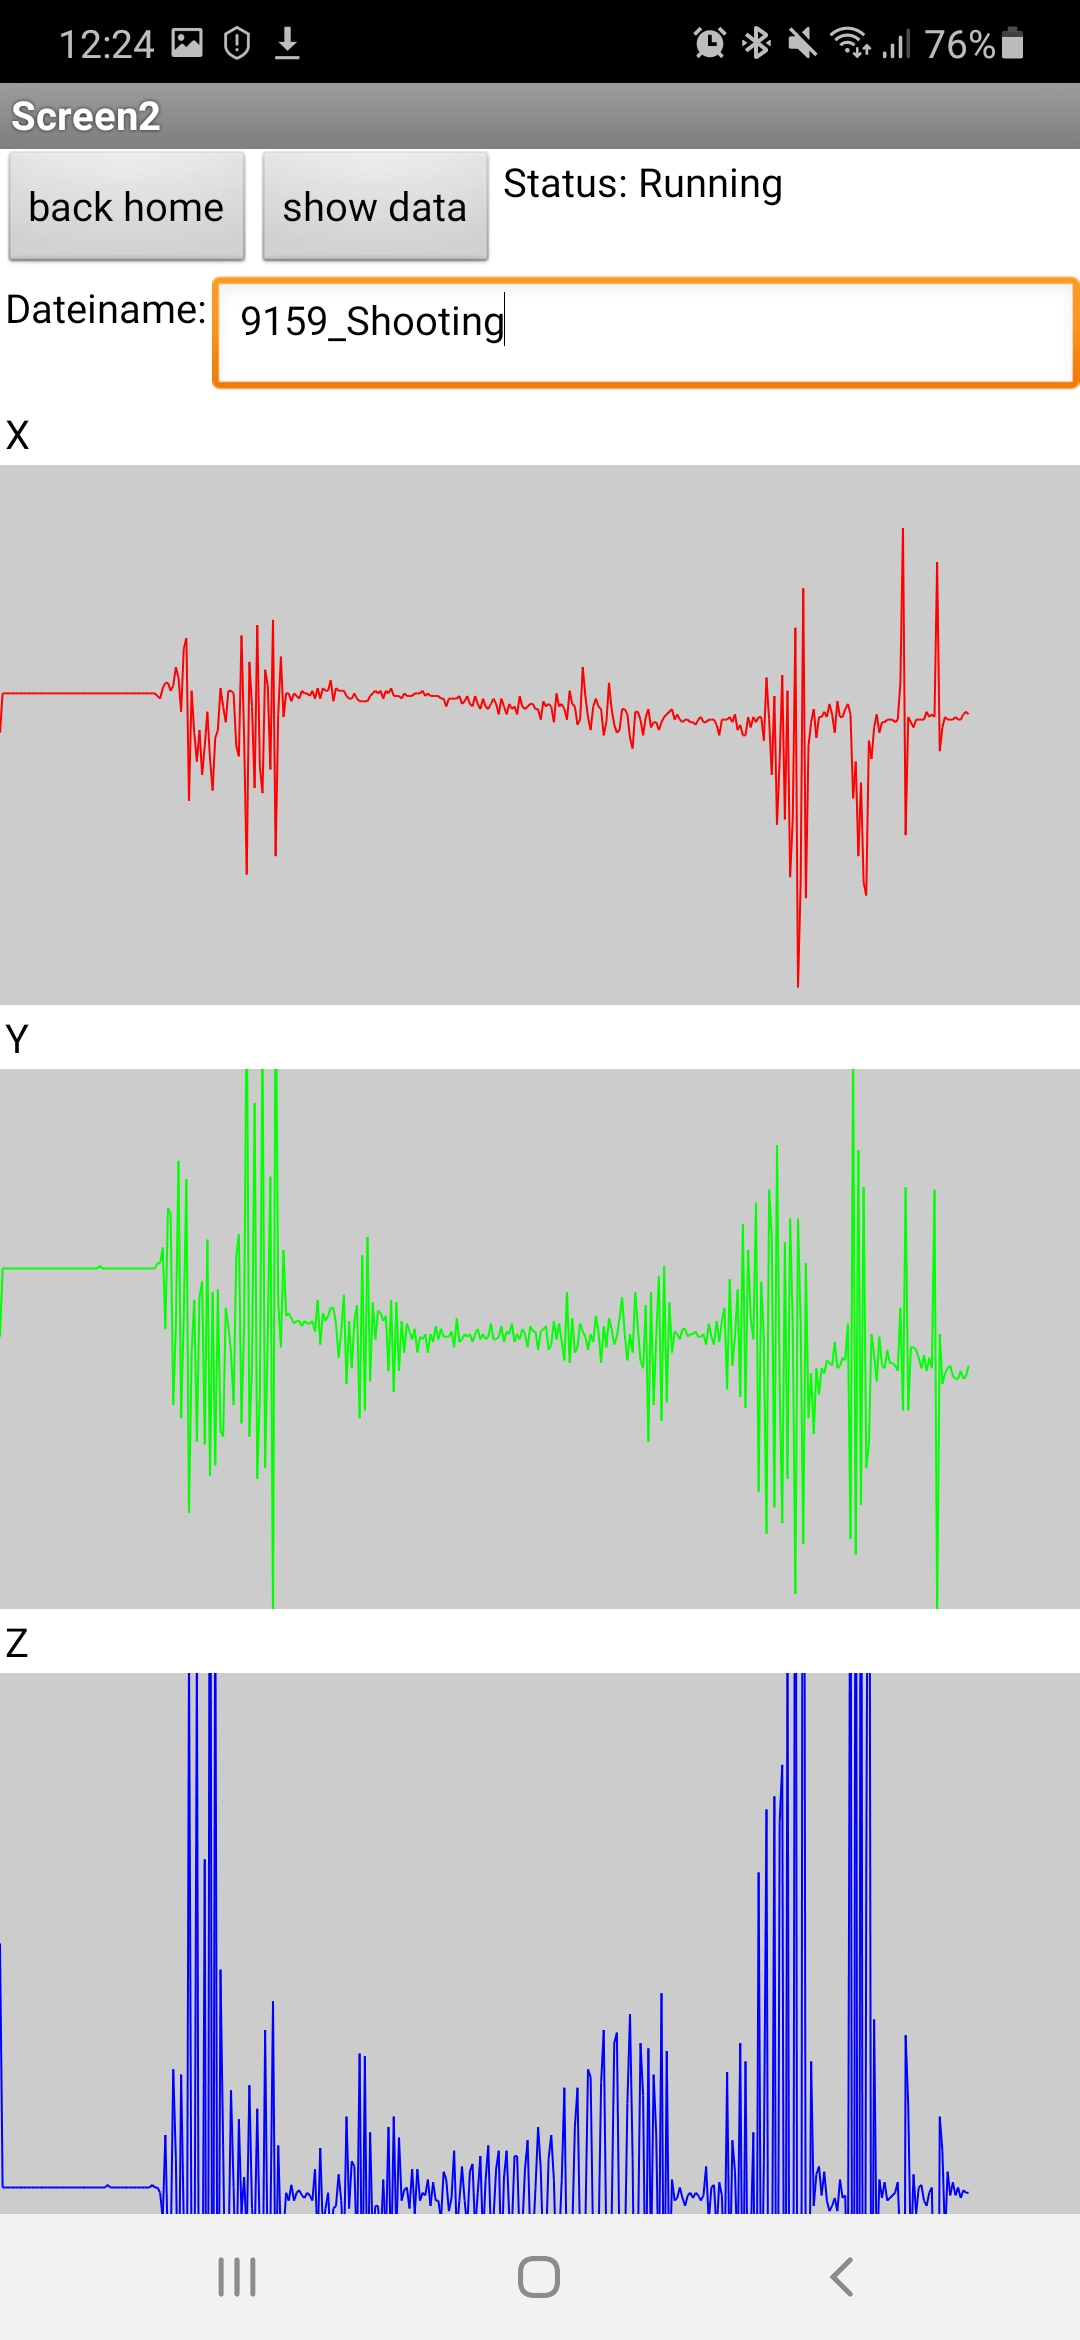
\includegraphics[height=10cm]{Bilder/GraphRec.jpg}
    \end{minipage}
    \hfill
    \begin{minipage}{0.5\textwidth}
        Die von den anderen Funktionen aufgezeichneten Funktionen können hier ausgegeben
        werden. Hierzu benötigt der Schütze den Namen der Datei. Die Dateien werden
        seit kurzem unter Android in einem App-Eigenem Ordner gespeichert. Diesen muss
        der Schütze momentan auslesen um den zufälligen Namen der neuen Datei zu kennen.\\
        Die Daten werden als Graph dargestellt. Die Beschleunigungsdaten werden außerdem
        in Rohform über dem Graphen ausgegeben.\\
    \end{minipage}

\section{Arduino Firmware}
Das Programm auf dem Arduino Nano 33 BLE stellt zu Beginn eine 
I$^2$C Verbindung mit dem MPU9250 her und startet das BLE-Modul.\\
Sobald ein Ger"at sich mit dem Arduino verbindet, beginnt dieser
mit der Datenübertragung.\\
Hierbei wurden die Filter vom Digital-Motion-Processor des MPU9250 
schon mit einem Low-Pass-Filter verarbeitet. 
\section{Gleichmäßige und ungleichmäßige Beschleunigung}
Um die Distanz aus der gemessenen Beschleunigung zu berechnen,
fand ich zwei verschiedene Formeln. Die wohl bekannteste Umrechnung 
benutzt Integrale, die zweite Formel ist die der gleichm"aßigen 
Beschleunigung.\\
\\
Die Integration wird von allen mir bekannten Forschungen verwendet. 
Man muss eine Doppelintegration
ausführen um von Beschleunigung auf Distanz zu kommen, hierbei verwandelt 
sich das Rauschen des Sensors in Drift und so einen exponentiell steigenden
Fehler. \\ 
Die gleichmäßige Formel kann im Gegensatz zum Integral, nur positive 
Beschleunigungen verwerten, hat in den folgenden Tests allerdings 
deutlich genauere Werte und einen geringeren Fehler bei Stillstand 
aufgezeigt. So wird in diesem Projekt die gleichmäßige Beschleunigungsformel 
verwendet.\\
\\
Als Zeit wird die Frequenz, mit der der Sensor Daten misst, 
genommen. Hierfür wird die Frequenz in Zeitabschnitte umgerechnet, mit 
der die Formeln letzendlich arbeiten.
\subsection{Gleichmäßige Formel}
Die Formel für gleichmäßige Beschleunigung berechnete 
die Distanz in meinen Versuchen mit einer Genauigkeit von
+-10 cm auf 30cm Teststrecke. Wurden hierbei ebenfalls 
negative Beschleunigungen gemessen wirkten sich diese direkt
auf die Distanz aus. Dies stellte ein Problem beim abbremsen
am Ende der Teststrecke dar. Die Werte sanken wieder auf null.\\
Aus diesem Grund sind nur positive Werte für diese Funktion 
zugelassen. Hier der Code-Aussschnitt aus der Berechnung.\\
Für die Tests wurde dieser Code statt der BLE-Übetragung 
auf dem Arduino ausgeführt.

\begin{verbatim}
    if (acc > 0) {
    t = (freq / 1000); //hz is not time but frequenzy

    distance = (distance) /*+ (velocity * t) */ + (acc * (t * t) * 0.5);
    velocity = acc * t;
    }
\end{verbatim}

\subsection{Integral}
Die Berechnung der Distanz über Integrale ist der Standard 
in der Wissenschaft, obwohl die Fehler die sie mit sich bringt
bekannt sind. Eben diese Fehler wirkten sich bei meinem Sensor
stark aus.\\
Die Testergebnisse ergaben einen Fehler von $\pm15$cm auf einer Strecke
von 30cm. Ebenso war das Ergebnis sofort in Centimetern, statt wie erwartet in Metern. 
Wurde der Sensor zurückbewegt an seinen Startpunkt sank
der Wert jedoch wieder auf Null ab. Somit kann man schließen,
dass das Ergebniss nur falsch skaliert ist.\\
Dieser Fehler wurde noch nicht behoben. \\
Ein klarer Vorteil dieser Rechnung zeigt sich schon beim Test,
die Formel funktioniert auch für negative Beschleunigungen.
Der Wert sinkt am Ende der Teststrecke nicht ab, sondern bleibt
auf seinem hohen Wert.\\
Folgend der Code-Ausschnitt der Integral-Rechnung:
\begin{verbatim}
    t = (freq / 1000); // hz to time

    velocity = t * ((acc + accOld) / 2) + velocity;
    accOld = acc;
    distance = t * ((velocity + velocityOld) / 2) + distance;
    velocityOld = velocity;  
\end{verbatim}
\subsection{Tests zu den Messungen}
\section{Distanz - Testaufbau}
Der Sensor wurde auf einem Breadboard mit einem Arduino Uno verbunden und übertrug die Werte
via USB-Kabel an den Seriellen Monitor der Arduino IDE. Um eine mögliche Schieflage auf dem
Breadboard abzufedern wurden aus 200 Messungen der Durchschnitt berechnet und von den Werten vor
der Verarbeitung subtrahiert. So liegt der Sensor mathematisch absolut flach auf. \\

\subsection{Distanzmessungen}
Insgesamt wurden 10 Tests pro Formel gemacht, die Ergebnisse können Sie unten einsehen.\\

\begin{figure} [h]
    \centering
    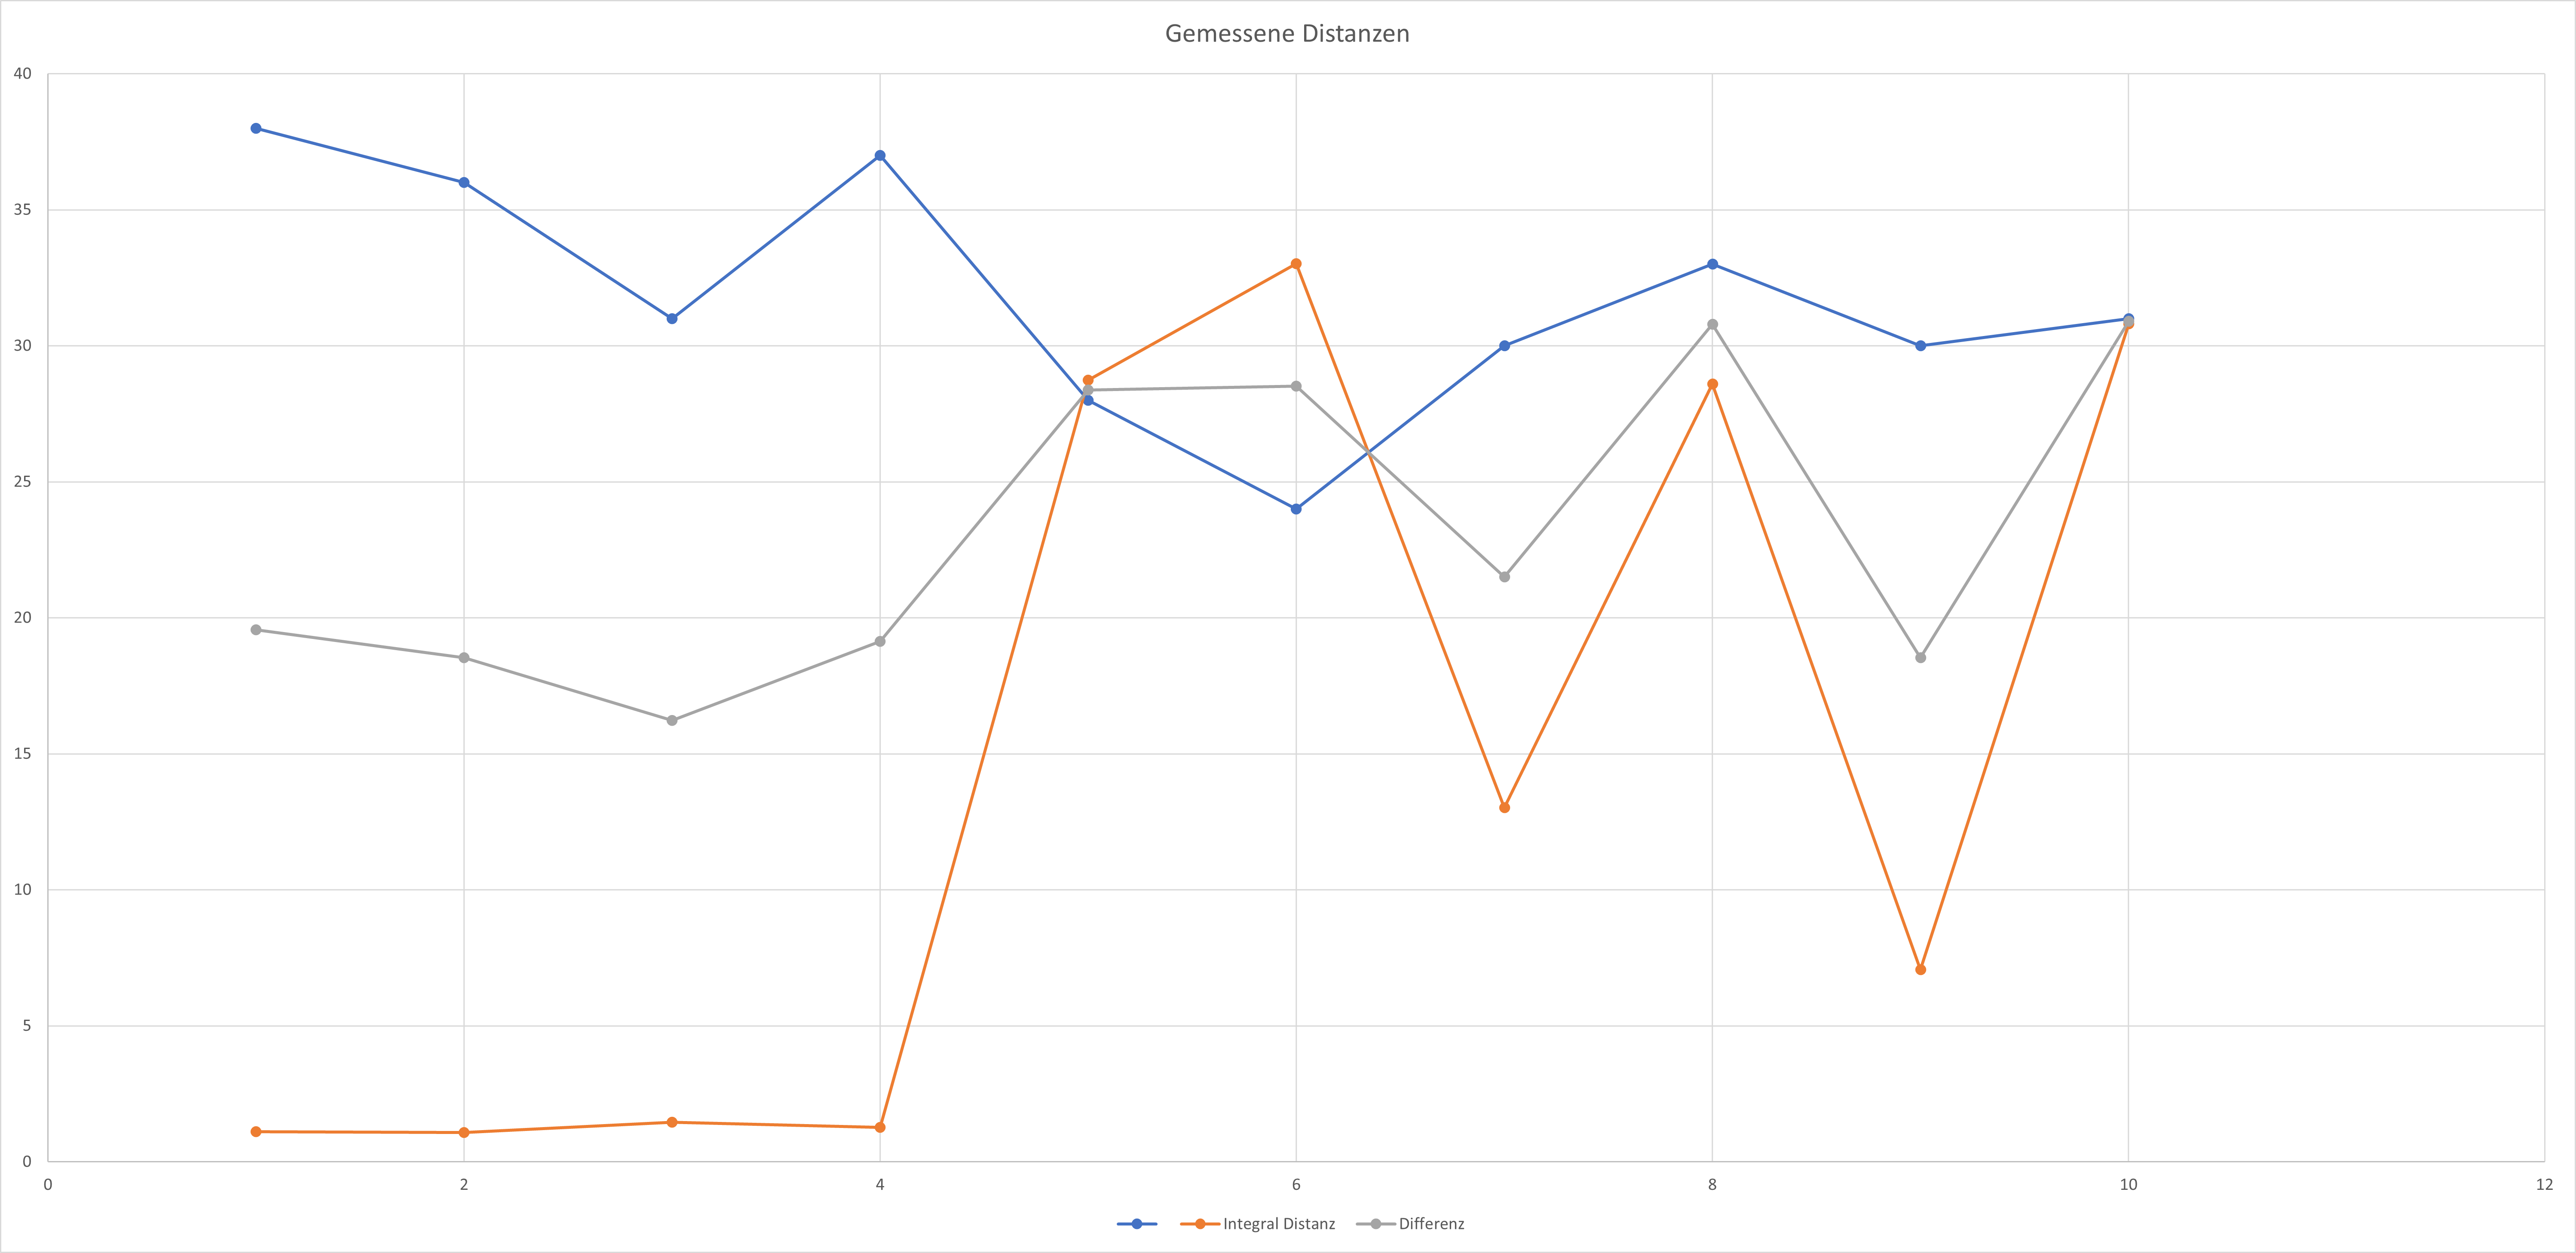
\includegraphics[width = 15cm]{Bilder/_DistanzVergleich}
    \caption{Distanzen | Alle Tests}
    %\label{fig:wo-bin-ich}
    \end{figure}

\subsection{Fehler}
Die zwei weiteren Graphen zeigen die Fehler bei 10 sek"undigem Stillstand. Der exponentielle Drift 
bei der Integralen Formel ist typisch.

\begin{figure} [h]
    \centering
    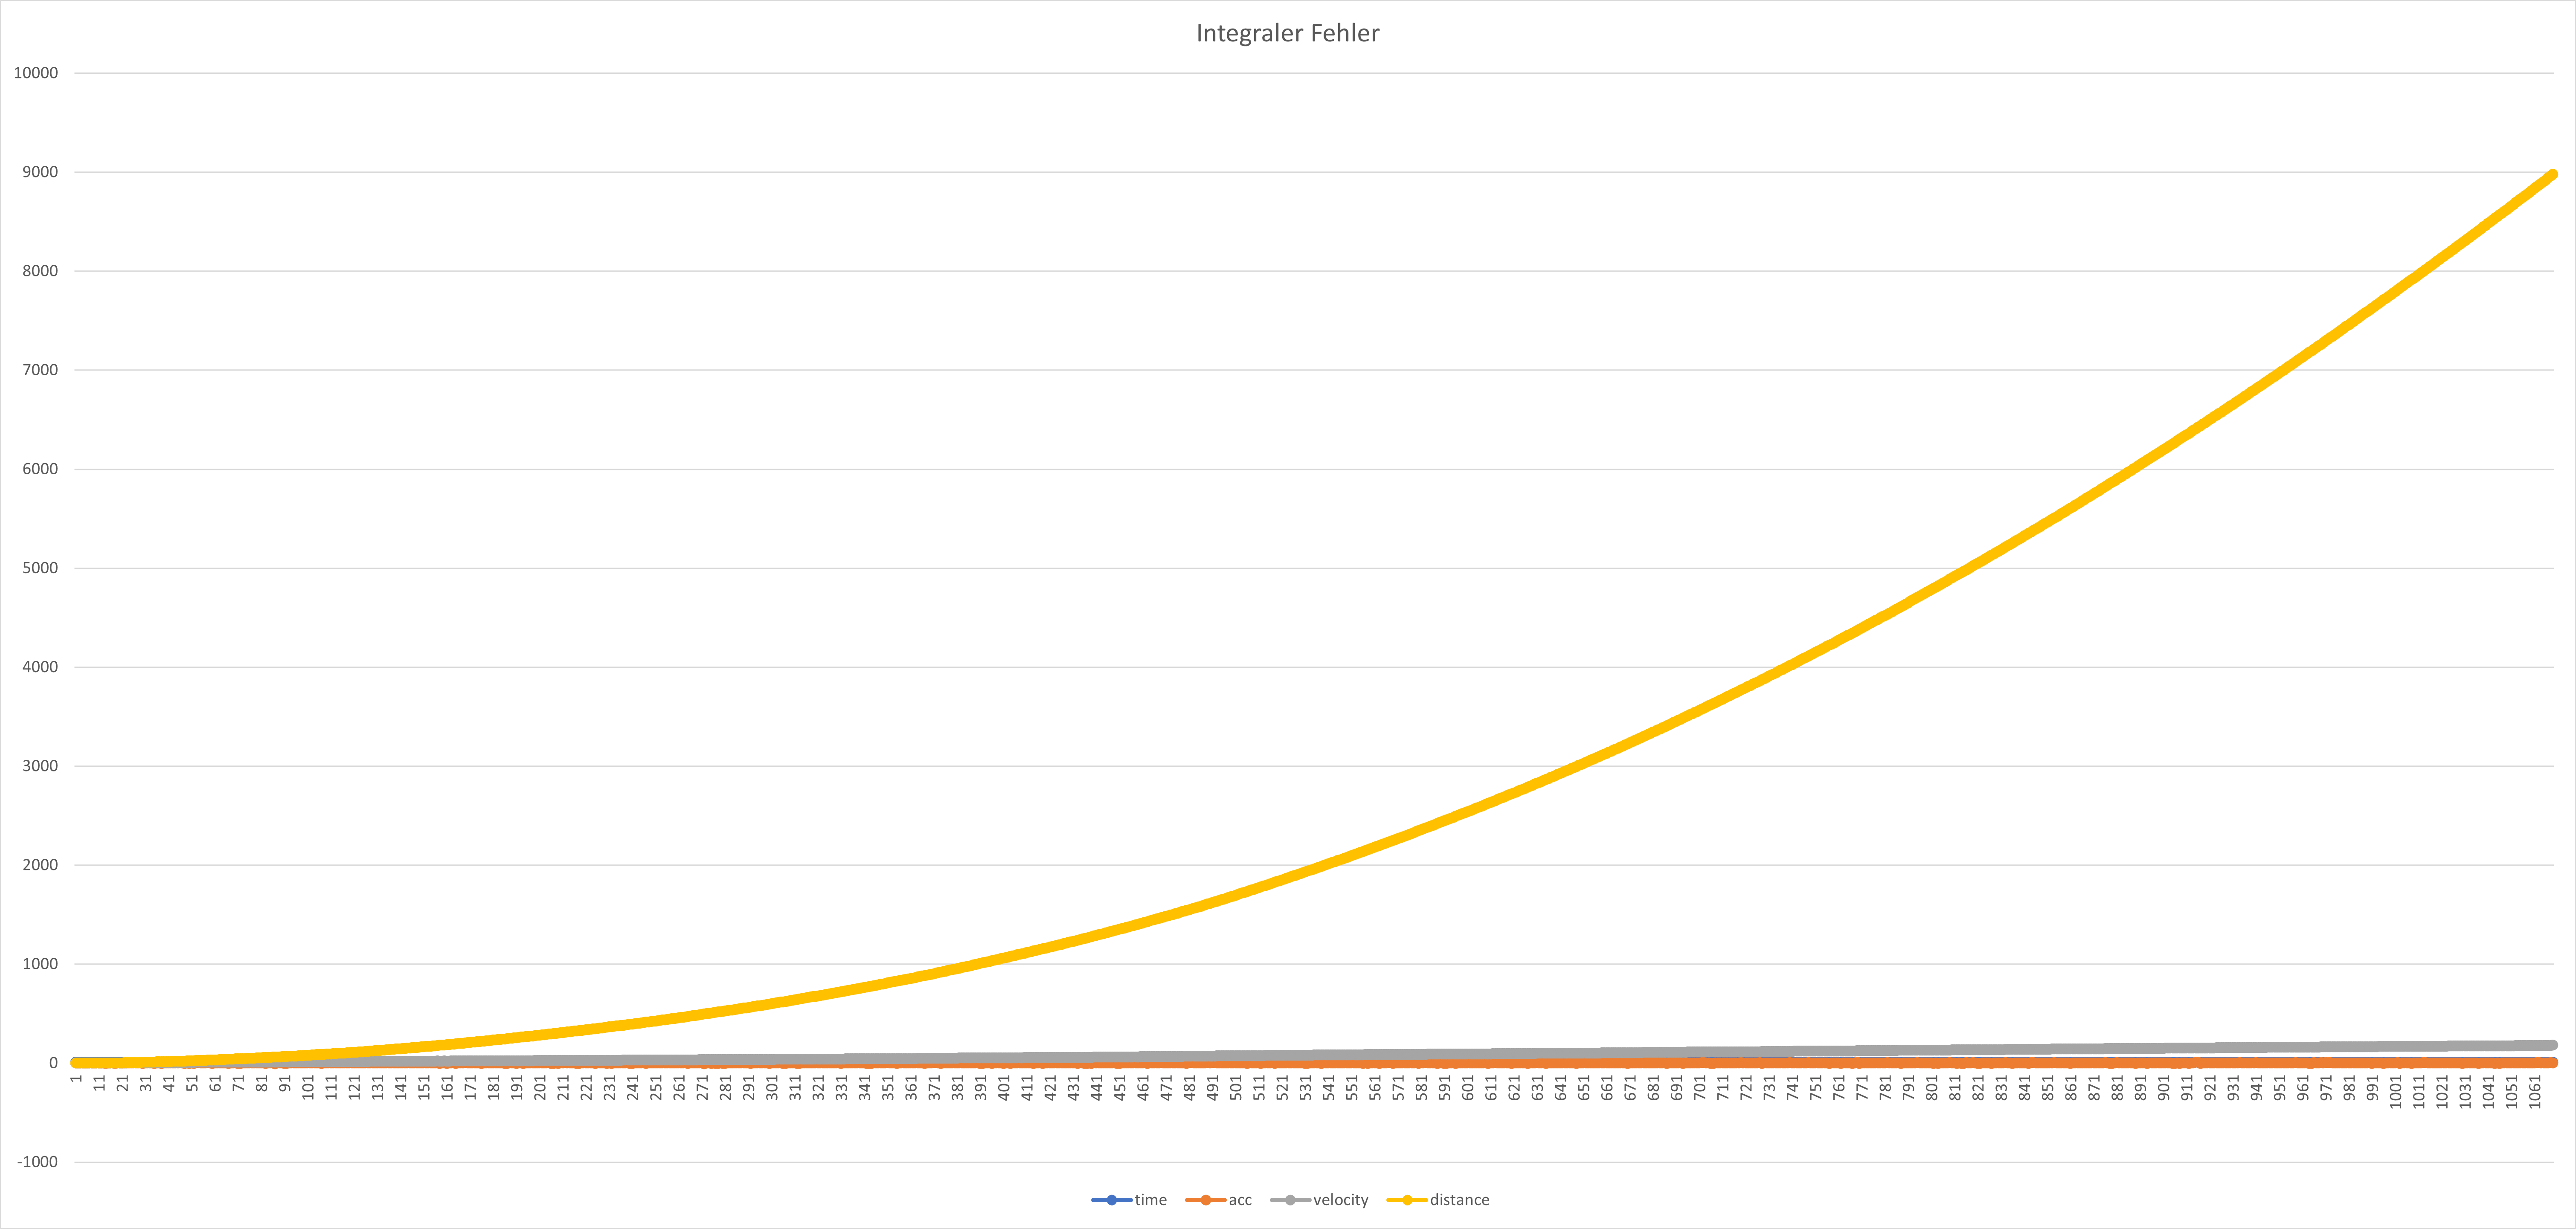
\includegraphics[width = 15cm]{Bilder/_integralDistance001}
    \caption{Integrale Formel | Drift}
    %\label{fig:wo-bin-ich}
    \end{figure}

    \begin{figure} [h]
        \centering
        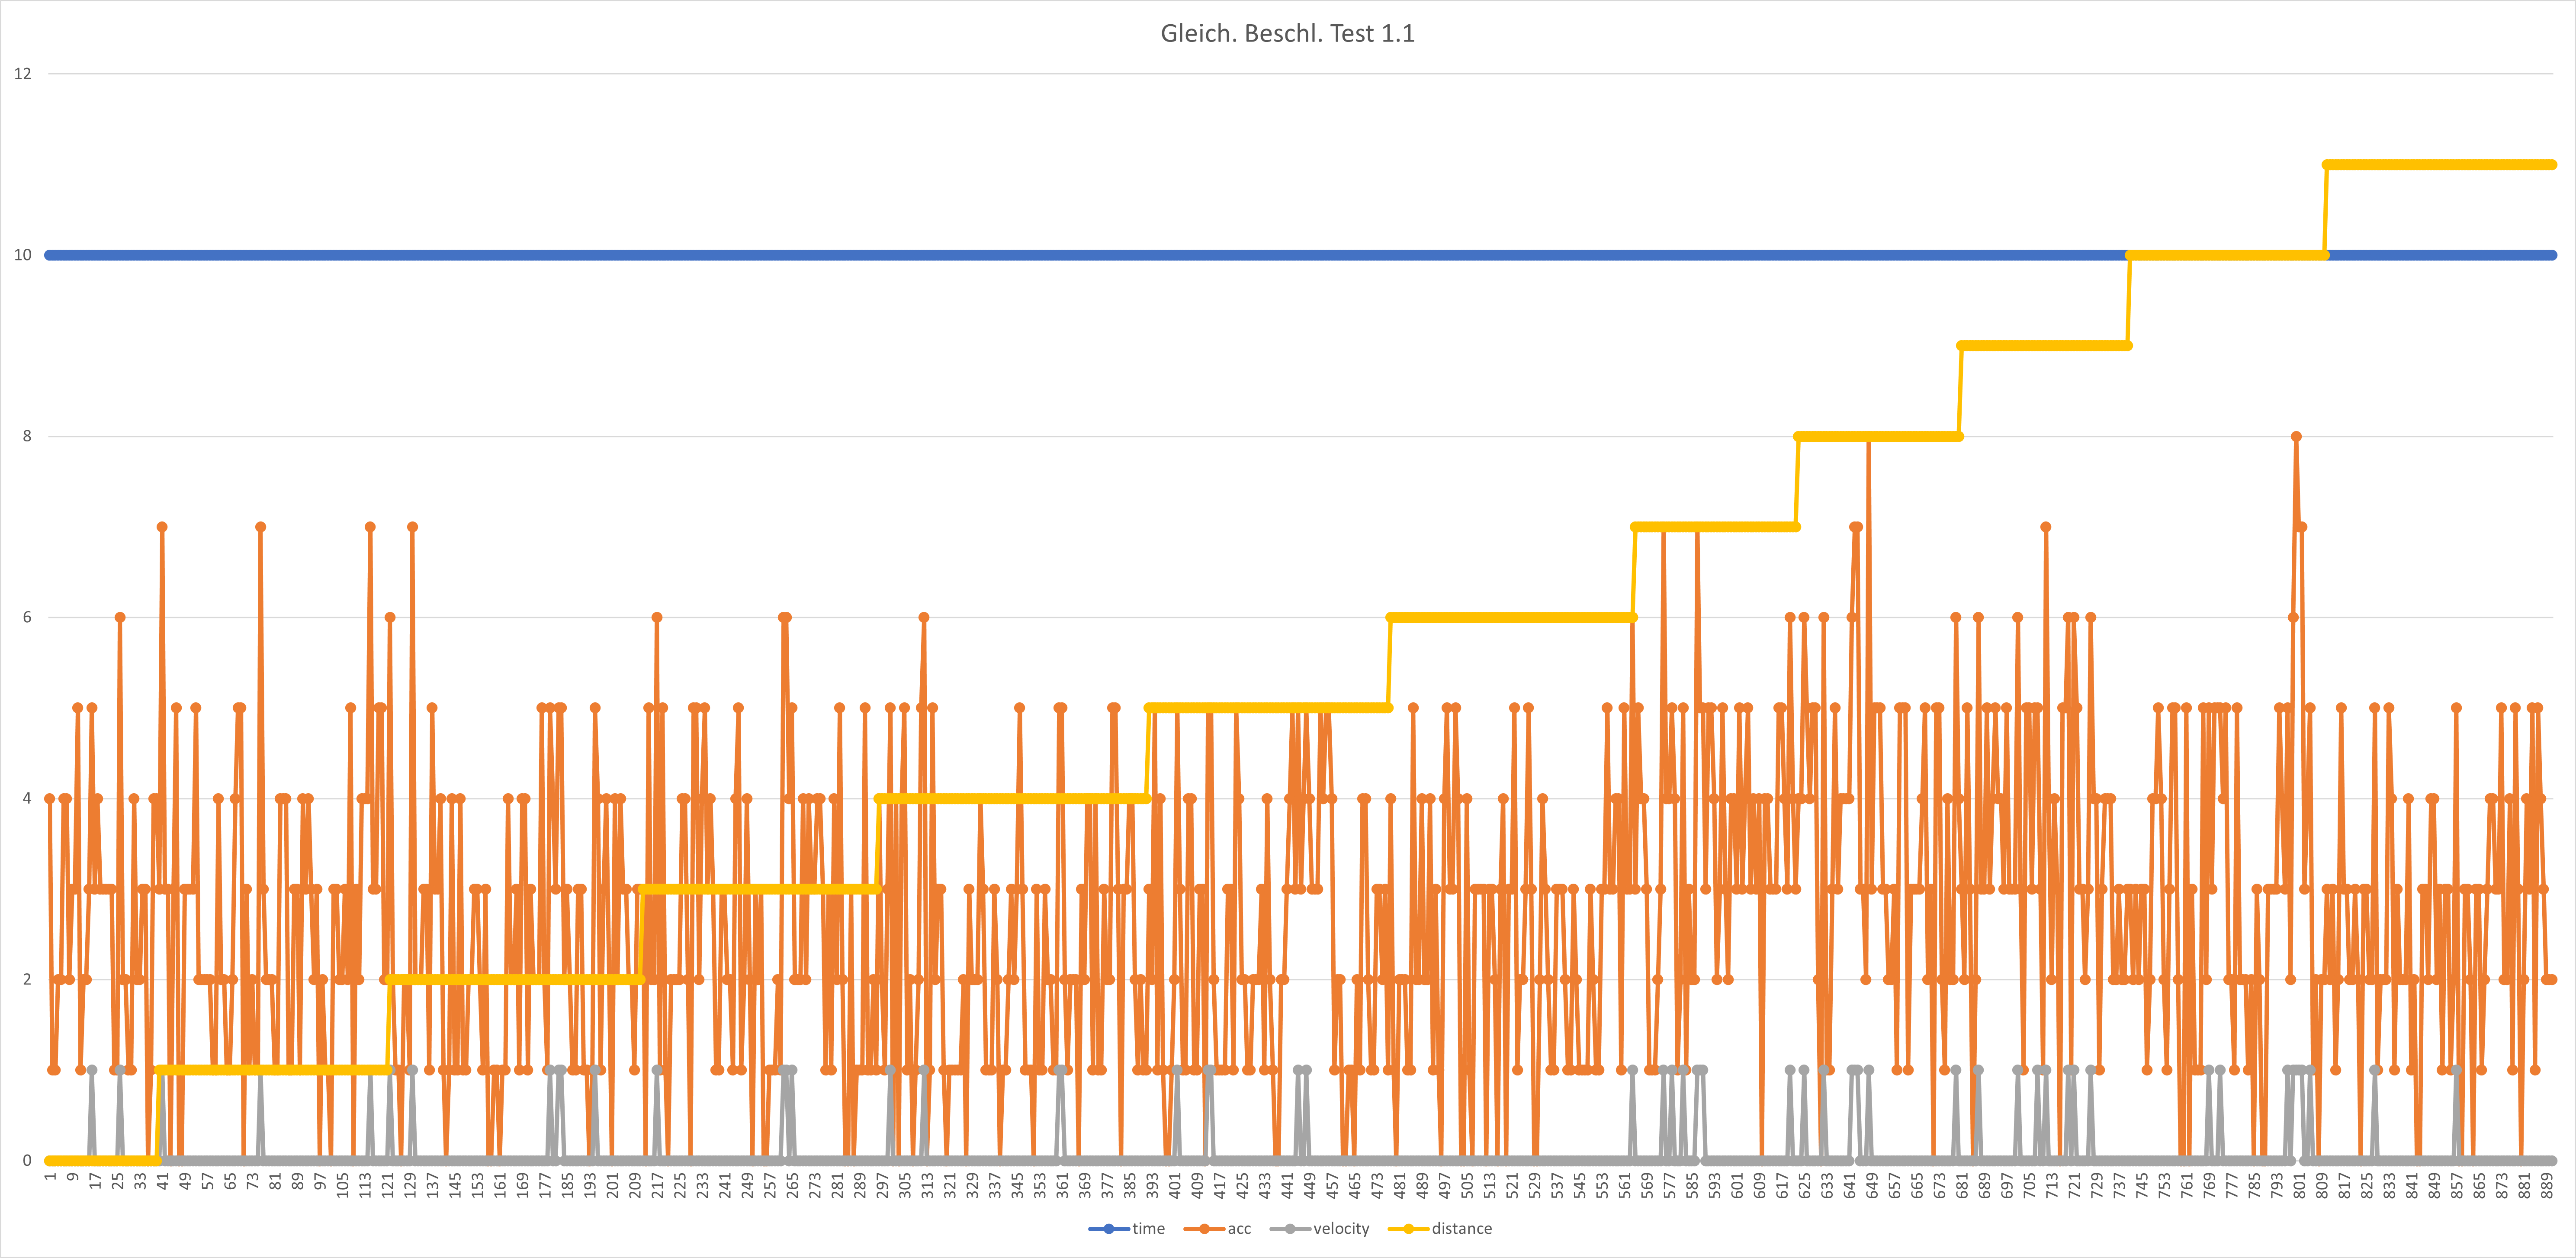
\includegraphics[width = 15cm]{Bilder/_constDistance001}
        \caption{Gleichf"ormige Beschl. Formel | Drift}
        %\label{fig:wo-bin-ich}
        \end{figure}
    


\chapter{Machine Learning}
\section{Datenauswahl und Dimensionen}
\input{MLData}
\section{Modell und Funktion}
\input{MLModNFunk}

\chapter{Fazit}
Die Distanzmessung über den MPU9250 funktioniert 
mit einem relativ großem Fehler, der es schwer macht
die Daten direkt in ein 3D-Programm einzufügen. 
Danke an \\
\begin{itemize}
    \item Herr Czernohous (Korrekturlesen der Arbeit und technische Hilfe, Kauf der Materialien)
    \item Herr Dierle (Hilfe bei physikalischen Zusammenhängen und Formeln, Korrekturlesen der Arbeit)
    \item Platzhalter
\end{itemize}
\bibliography{bibliography}
\bibliographystyle{plain}
\end{document}
